\section{Experimental setup}

In this section I will schematically present the experimental setup used for this thesis.
Note however that, being this an experimental work, the setup changed various times and it is difficult to give a complete description of it, for all the states it had.

The schematics presented here correspond to the final setup.

\subsection{Cryostat}

Since the qubits that we are considering are transmons, they work exploiting the superconductivity phenomenon.
To reach the superconductivity regime, we need a device capable of refrigerating it to the mK region.
The device employed for this task is called cryostat.

In this thesis I used both the SD and XLD cryostats manufactured by Bluefors, but the majority of the data presented here was acquired with qubits in the XLD so I will focus on the description of those last setups.

The technique used by cryostats to achieve these temperatures is the dilution refrigeration~\cite{McClintock2003, Craig2004}: a process that exploit a mixture of $^4\mathrm{He}$ and $^3\mathrm{He}$ to reach temperatures below the minimal one achievable through pressure process.
The two isotopes are quite different: the former is a boson with spin $0$ that can be found in natural gas reservoirs, while the latter is a fermion (spin $1/2$) and is the byproduct of tritium fabrication in nuclear reactors.

$\mathrm{^3He}$ can be diluted in $\mathrm{^4He}$ at any concentration, but when the mixture is cooled below $\sim 0.85$ K (note that pure liquid $\mathrm{^3He}$ can be cooled to a minimum of $0.3$ K) it undergoes a spontaneous phase separation.

Two phases now coexist: a concentrated phase composed essentially only of $\mathrm{^3He}$ and a diluted phase that, on the contrary, is mostly composed of $\mathrm{^4He}$.

\begin{figure}[ht]
    \centering
    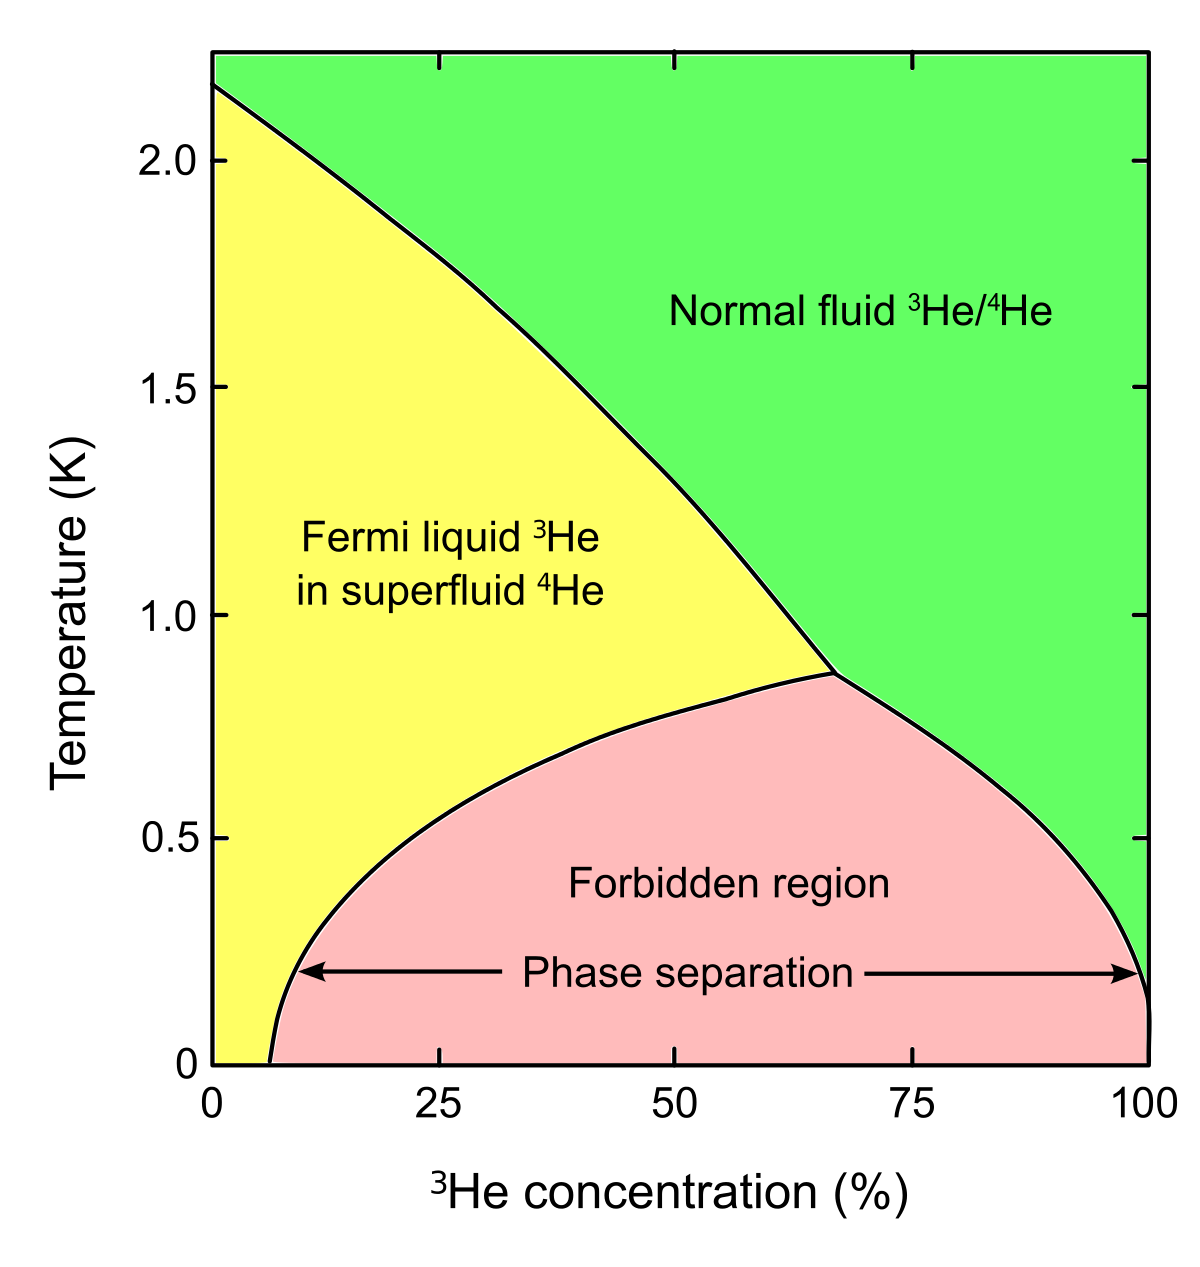
\includegraphics[width=0.6\textwidth]{Setup-software/figures/Helium_phase_diagram.svg.png}
    \caption{Phase diagram for $\mathrm{He}$ as a function of $\mathrm{^3He}$ concentration.}
    \label{fig:cryostat:heliumphasediagram}
\end{figure}

The graph in \cref{fig:cryostat:heliumphasediagram} shows equilibrium concentrations: intersections of the phase separation line and a horizontal isotherm line correspond to the concentrations of the two different phases (if below the $0.85$ mK threshold).

In the coldest part of the cryostat, the mixing chamber, $\mathrm{^3He}$ atoms cross the interface between the concentrated and the diluted phase.
This transition is endothermic and removes heat from the mixing chamber.
When $\mathrm{^3He}$ dissolves in $\mathrm{^4He}$ at such low temperatures, it undergoes a process similar to evaporation in a vacuum and produces vapor.
The diluted phase is connected to another chamber called still (short for distilling pot) that is held by a heater at $\sim0.7$ K and continuously pumped to remove the vapor which is mainly composed of $\mathrm{^3He}$ because of its greater vapor pressure.
The depletion of $\mathrm{^3He}$ within the still produces an osmotic pressure that drives more $\mathrm{^3He}$ to the still from the mixing chamber where phase transition can continue to happen.
$\mathrm{^3He}$ pumped from the still is reintroduced to the mixing chamber through a flow impedance that enables the helium to condense and that cools it down via heat exchangers that work making use of the cold $\mathrm{^3He}$ that is flowing upwards toward the still. This process is schematized in \cref{fig:cryostat:heliumdilutionrefrigerator}.

In \cref{fig:xldcryostat} some picture of the XLD are present.
Without any thermal load can reach $8$ mK, while with minimal thermal load (the qubits mounted but not probed) is stable at $9$ mK.

\begin{figure}[H]
    \centering
    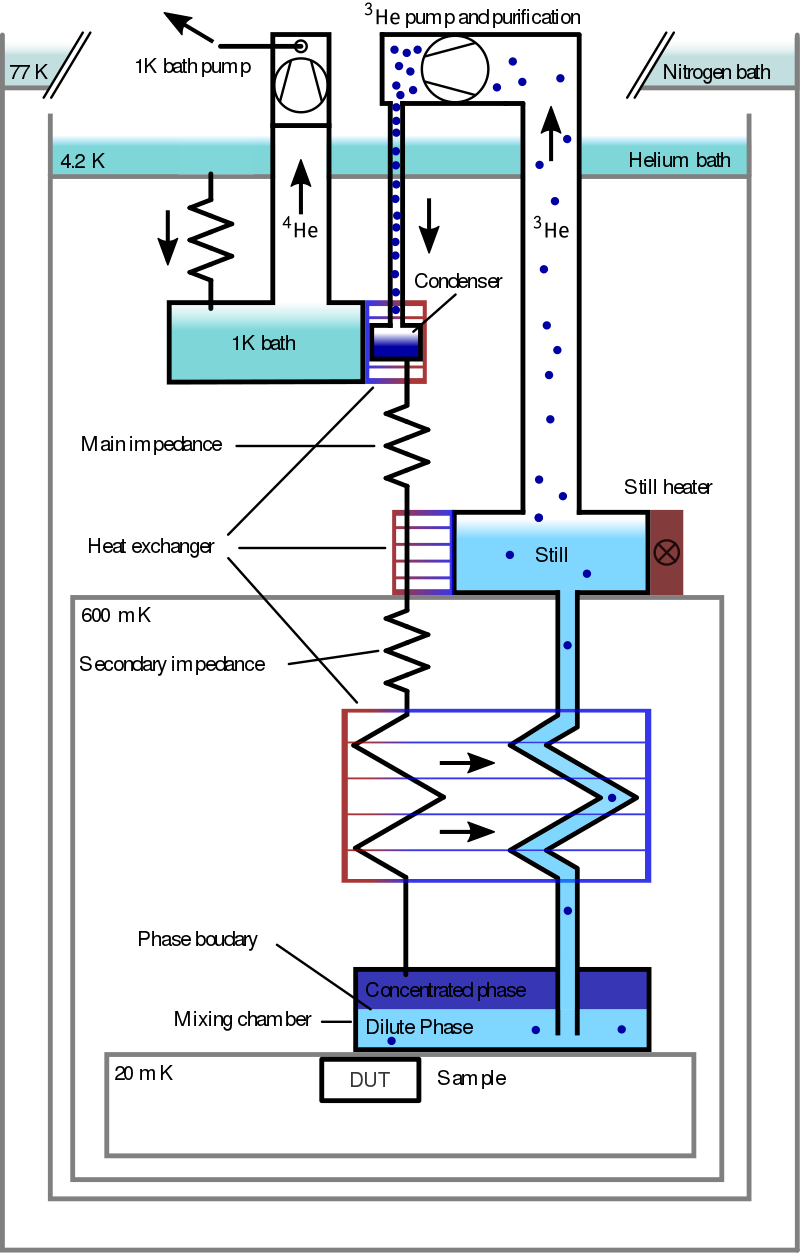
\includegraphics[width=0.6\textwidth]{Setup-software/figures/dilution_refrigerator.png}
    \caption{Outline of the dilution process.}
    \label{fig:cryostat:heliumdilutionrefrigerator}
\end{figure}


\begin{figure}[ht]
    \centering
    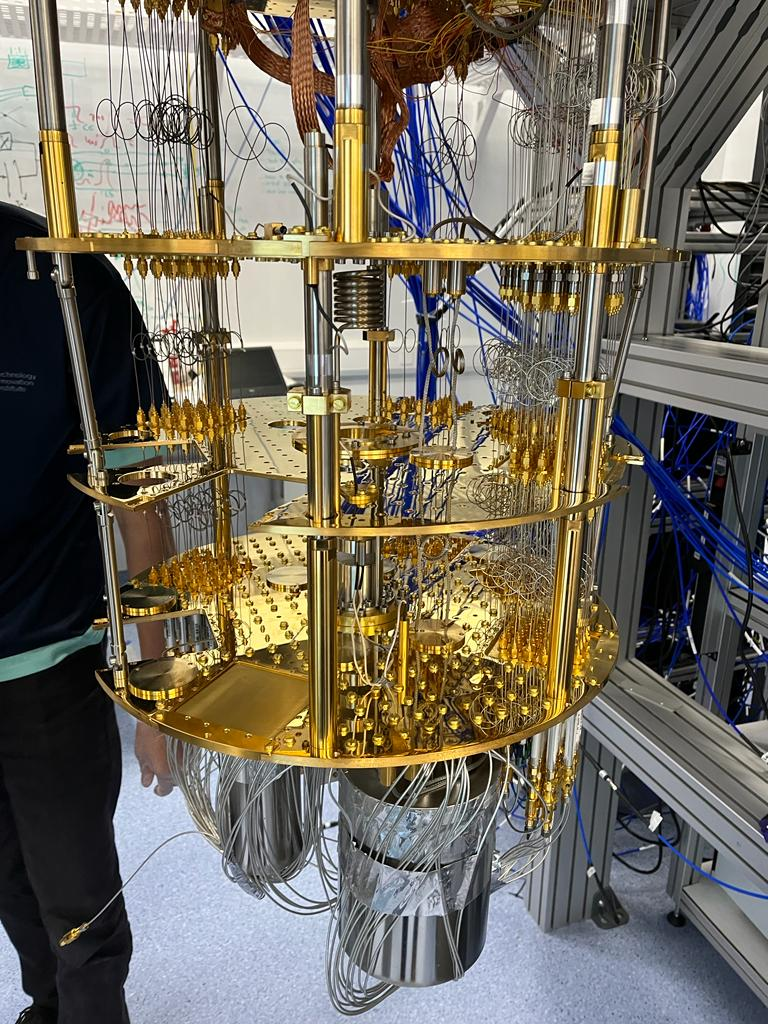
\includegraphics[width=0.55\textwidth]{Setup-software/figures/XLD.jpeg}
    \caption{Bluefors XLD.}
    \label{fig:xldcryostat}
\end{figure}

\subsection{FPGA \& RFSoC}

A Field-Programmable Gate Array (FPGA) is an electronic board that supports complete firmware configuration \textit{after} manufacturing as well as partial re-configurations while executing a specific program.\\
While integrated circuits serve a specific purpose and cannot be re-configured after fabrication, FPGAs can contain arrays of programmable logic blocks that can serve simple logic purposes (as Boolean operations) or complex functions, depending on the loaded firmware.
Since they are completely re-configurable and since they can improve the performance of standard CPU (with task-specific firmwares) without the large energy conception required by GPUs, FPGAs are rapidly becoming of widespread use.
Moreover, since the same FPGA can serve different purposes in extremely different fields, it is usually a cheap alternative to standard systems.\\
The drawback of all of this is in the overhead that programming a FPGA introduces.
To compile a FPGA firmware one first has to define the logic to use via Hardware Description Languages (HDL) then design the connections internal to the FPGA logic and conduct precise tests on the produced firmware.

The type of FPGAs used in my thesis are RFSoC, namely Radio Frequency System on Chip: their main characteristic is the capability of synthesizing directly frequency up to $\approx 10$ GHz, as well as the capability of acquiring extremely high frequency by exploiting the downsampling technique. 
All of this combined in the same board, along with a standard CPU, RAM and memory: enabling the creation of a full on-board system.\\
In this section I will provide some explanation on the techniques used for high-frequency synthesis and high frequency acquisition. 
Also, some details on the FPGAs used will be provided.

\subsubsection{Direct Digital Synthesis (DDS)}
The technique used for direct microwave synthesis is called \textit{Direct Digital Synthesis} (DDS) and it enables to use the DACs as arbitrary waveform generators for high frequencies~\cite{DDS}.

In general, a DDS system consist in a precision reference clock (often a crystal clock), an address counter, a programmable read-only memory (PROM) and a DAC (see \cref{fig:simple_DDS} for reference).\\
In the PROM, a complete cycle of a periodic function is stored and the address counter steps through it, accessing sequentially  all the PROMS's memory locations (so the PROM is working a lookup table).
The DAC then converts the input from the PROM, to analog outputs.

Note also that the PROM can be composed of two different lookup tables, for complex I-Q signals, often referred to "in-phase and quadrature signals," are a pair of time-varying signals used in signal processing and communications. They represent:
\begin{description}
    \item[In-Phase (I) Component] The "I" component represents the signal's amplitude or phase information. It corresponds to the real part of the complex signal.
    \item[Quadrature (Q) Component] The "Q" component is also a real part of the complex signal but is phase-shifted by 90 degrees relative to the "I" component. The "Q" component carries information orthogonal to that of the "I" component.
\end{description}


\begin{figure}[ht]
    \centering
    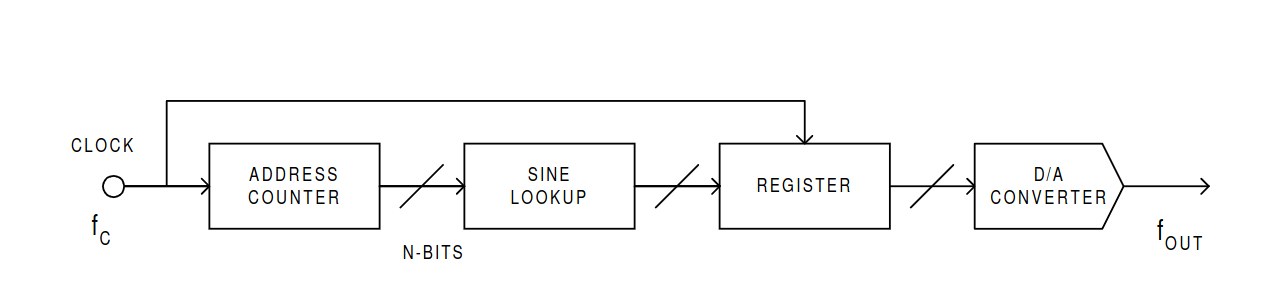
\includegraphics[width=\textwidth]{Setup-software/figures/simple_DDS.png}
    \caption{A simple Direct-Digital-Synthesizer, where the function stored in PROM is a sine wave. Credits~\cite{DDS}.}
    \label{fig:simple_DDS}
\end{figure}

This implementation of DDS is a bit simplified and, although it works, it lacks tuning flexibility and the output frequency is effectively fixed to the reference clock one.\\
A modern DDS system adds to the shown signal chain a phase accumulator, creating an architecture usually referred to as numerically-controlled oscillator NCO (see \cref{fig:phase_accumulator_DDS}).
\begin{figure}[ht]
    \centering
    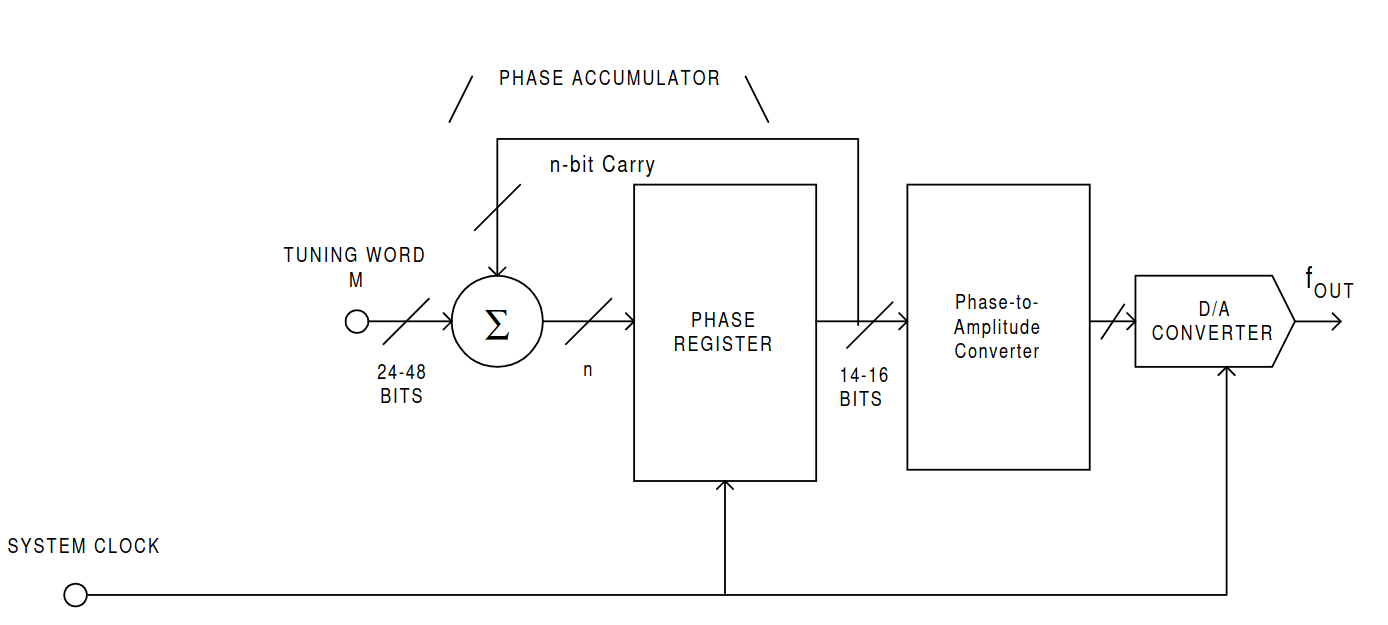
\includegraphics[width=\textwidth]{Setup-software/figures/phase_accumulator_DDS.png}
    \caption[Details of the phase accumulator component of a DDS system]{Details of the phase accumulator component of a DDS system. Credits~\cite{DDS}.}
    \label{fig:phase_accumulator_DDS}
\end{figure}
The address counter is replaced with an N-bit variable-modulus counter and a phase register: effectively storing not a "random" real number, but an integer mapped to a "phase wheel" that indicates the function points to be generated. A typical scheme is presented in \cref{fig:DDS}.

\begin{figure}[ht]
    \centering
    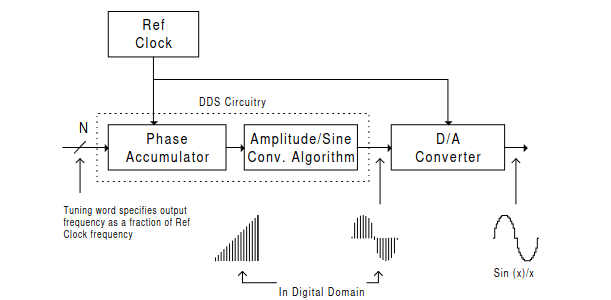
\includegraphics[width=\textwidth]{Setup-software/figures/DDS.png}
    \caption[Scheme of a generic NCO DDS system]{Scheme of a generic NCO DDS system. Credits~\cite{DDS}.}
    \label{fig:DDS}
\end{figure}

This architecture, in respect to the more standard \textit{Phase-Locked Loop} (PLL), offers the advantages of micro-Hertz tuning resolutions, unparalleled matching and control of I-Q synthesized outputs, extremely fast changing speed in frequency and phase.


\subsubsection{Aliasing and synthesis at higher Nyquist zones}\label{sec:aliasing}
Now that we have an idea of the hardware involved for the synthesis, let's try to understand analytically how the DACs behave, how can they be used to synthesize directly in the microwave region, and what are some of the problems involved. 

We can write the output of the DACs as an analytical function~\cite{Kalfus2020}.
Given $f_s$ the sampling frequency, so the rate of conversion from digital samples of a generic analytical function $x(t)$ to analog outputs $v(t)$, we can write:
\begin{equation}\label{eq:v(t)_DAC}
    v(t) = \left[ x(t) \sum^\infty_{k=-\infty} \delta (t - kT) \right] * r(t)
\end{equation}
Where $T=1/f_s$ is the sampling period, inverse of the sampling frequency, and $*$ is the convolution in time operator.
The $r(t)$ function is called \textit{reconstruction waveform} and describes the DAC behaviour between two subsequent samples (so it is non-zero only for $0\le t \le T$).
So, trying to understand \cref{eq:v(t)_DAC}, the summation if a function that is always zero, but in multiples of $T$, where the value between brackets reproduces the $x(t)$ function. Then we have to "connect the dots" to reach an analog continuous function, and this is the role of $*r(t)$.

We now apply Fourier Transform to $v(t)$ to obtain the frequency spectrum (capital functions are the FT of the corresponding time domain function):
\begin{equation*}
    V(\omega) = \mathcal{F}\{v(t)\}=\left[X(\omega) * \mathcal{F} \left\{\sum^\infty_{k=-\infty} \delta (t - kT)  \right\}\right] R(\omega)
\end{equation*}
For the sum we can recognize the $T$ periodicity:
\begin{equation*}
    \sum^\infty_{k=-\infty} \delta (t - kT)  = \sum^\infty_{n=-\infty} c_n e^{2\pi n / T}
\end{equation*}
From $k=0$ we can extract:
\begin{equation*}
    c_n = \frac{1}{T}\int^{T/2}_{T/2} \delta(t) e ^{2\pi n / T}dt = \frac{1}{T}
\end{equation*}
So we can compute the remaining part of FT:
\begin{equation*}
    \mathcal{F} \left\{\sum^\infty_{n=-\infty} \frac{1}{T} e^{2\pi n / T}  \right\} = \frac{1}{T}\sum^\infty_{n=-\infty}\delta (\omega - 2\pi n / T) = \sum^\infty_{n=-\infty} \delta (\omega T - 2\pi n)
\end{equation*}
And finally:
\begin{equation}
    V(\omega) = R(\omega) \left[ X(\omega) * \sum^\infty_{n=-\infty} \delta ( \omega T - 2\pi n) \right]
\end{equation}

The summation represents a series of peaks at multiple of the sampling frequency $f_s$ and the convolution with $X(\omega)$ creates copies of the original signal spectrum at each peak.
If $X(\omega)$ has a bandwidth larger than $f_s/2$ these copies will overlap, leading to a noise phenomenon called \textit{aliasing}.
The frequency bands to be considered, each extending for $f_s/2$, with the first starting at $0$ are called \textit{Nyquist zones}.
So it is not possible to synthesize a signal in a single zone: if $X(\omega)$ is confined in a single one, then every odd zone will have an identical image of the signal, while every even zone will have an inverted image.\\
This is why we generally need to use band pass filters: to exclude the images of spurious Nyquist zones and reduce aliasing effects.

The reconstruction waveform $r(t)$ manifest itself as a frequency-dependant attenuation and different functions will be used for maximize the output power for different Nyquist zones. In particular, the three most common choices are (note that they are all defined in the interval $[0\le t \le T]$):
\begin{description}
    \item[non-return-to-zero (NRZ):] $r(t) = 1\rightarrow R(\omega)=Te^{-i\omega T / 2}\ \frac{\sin\left(\omega T / 2\right)}{\omega T / 2}$
    \item[return-to-zero (RZ):] $r(t) = \theta (-t+0.5T)\rightarrow R(\omega) = \ \frac{T}{2}e^{-i\omega T/4} \ \frac{\sin(\omega T / 4)}{\omega T / 4}$\footnote{$\theta$ is the Heaviside function.}
    \item[mix-mode-rf (MIX):] $r(t) = -sign(t - 0.5T) \rightarrow R(\omega) = \ \frac{\omega T^2}{4}e^{-\ \frac{i}{2}(\omega T - \pi)}\left(\ \frac{\sin(\omega T / 4)}{\omega T / 4}\right)^2$
\end{description}

In \cref{fig:dac-modes} it is shown the attenuation-frequency dependence for different Nyquist zones and different reconstruction waveforms.

\begin{figure}[ht]
    \centering
    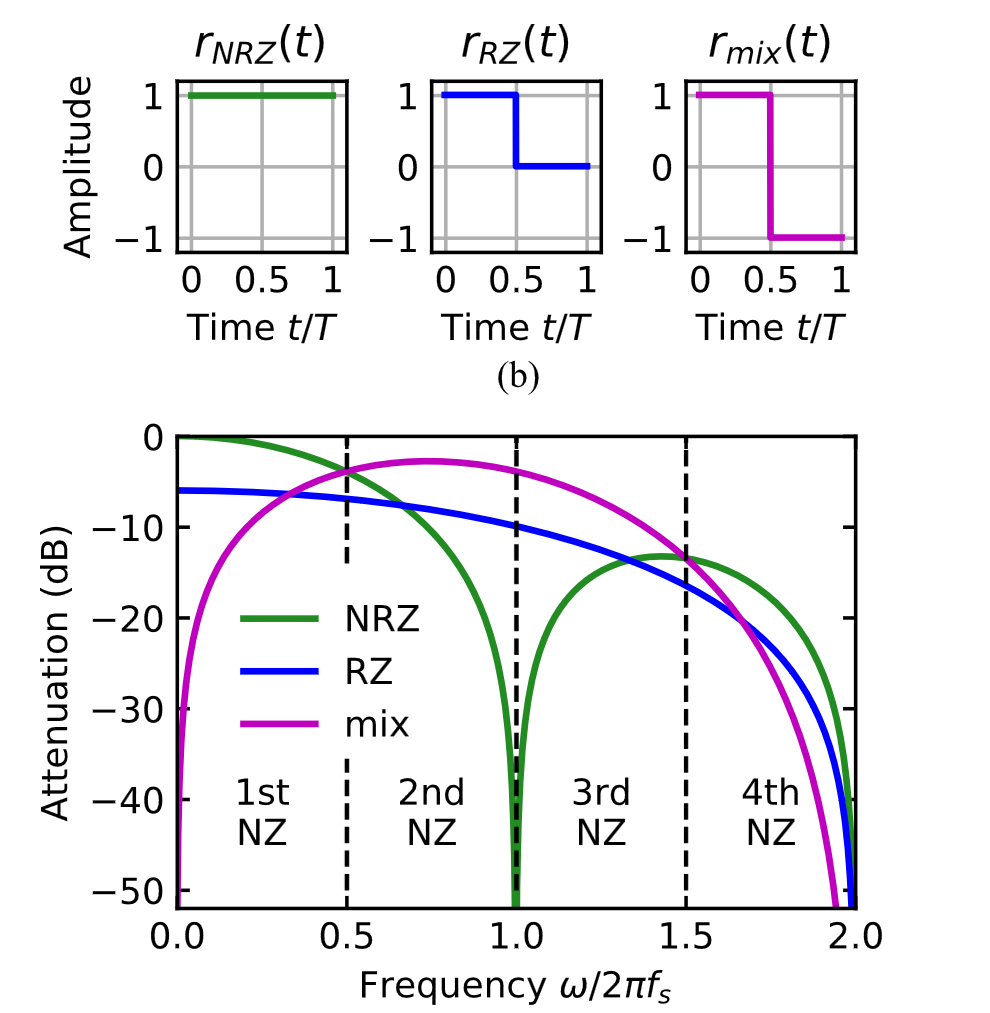
\includegraphics[width=0.6\textwidth]{Setup-software/figures/DAC_modes.png}
    \caption[Attenuation-frequency relationship at different Nyquist zones, for different reconstruction waveforms]{Attenuation-frequency relationship at different Nyquist zones, for different reconstruction waveforms. Credits~\cite{Kalfus2020}.}
    \label{fig:dac-modes}
\end{figure}

The RFSoC-based system that I developed used RNZ for the first Nyquist zone and MIX for all the others.

\subsubsection{Undersampling, decimation and Direct Down Conversion (DDC)}

In last section we saw the main principles and ideas that enable high-performance digital-to-analog conversion, now let's illustrate analog-to-digital.

The starting point for this discussion is the Nyquist-Shannon sampling theorem that establish a sufficient condition for a discrete-time signal to capture all the information contained in a continuous-tine signal.
Without entering in any details regarding the mathematical demonstration, we can express the theorem as\footnote{This theorem is often simply referred to as Nyquist sampling theorem.}:
\begin{theorem}
    If a function $x(t)$ does not contain any frequencies higher than $M$ Hz, then it can be completely described by finite samples spaced less than $1/(2M)$ s.
\end{theorem}
So, a signal must be sampled at a rate greater than twice its maximum frequency in order to assure complete and unambiguous reconstruction.
In general, the effect of not meeting the Nyquist-Shannon criterion is again aliasing.\\
Sampling with a frequency $\ge 2M$ is called \textit{normal sampling} or \textit{oversampling}.

If we use sampling frequency that are less than twice the maximum frequency than we use \textit{undersampling}.
Here we have another theorem, also called Nyquist-Shannon sampling theorem:
\begin{theorem}
    If a function $x(t)$ has a bandwidth of $B$ Hz, then it can be completely described by finite samples spaced less than $1/(2B)$ s.
\end{theorem}
The two theorems are similar, but note that they apply at the same time, so we will have aliasing.
While aliasing usually is a non-desired effect, with undersampling we try to exploit it.
The aliased signal always appear at:
\begin{equation}\label{eq:undersampling}
    f_{ADC} = f_s - f_{in}
\end{equation}
where $f_s$ is the sampling frequency, $f_{in}$ the input frequency and $f_{ADC}$ the acquired one.
If we know in advance that the signal is aliased, than we can easily recover the actual frequencies using the inverse of \cref{eq:undersampling}.

Since in our system we are acquiring a reflected/transmitted signal that was produces by us, we know exactly what frequencies we have in input and is very easy to reconstruct the signal.
Also note that the undersampling technique has several advantages:
\begin{itemize}
    \item higher sampling rate increases data rates to FPGAs and this can deteriorate performances or increase the cost of the FPGAs;
    \item higher data rates usually need more time to setup, meaning larger dead times;
    \item higher sampling rate are linked to higher power consumption;
    \item to reach a situation where the Nyquist-Shannon criterion is met we usually need to involve external Local Oscillators and Mixing, that are not needed for undersampling.
\end{itemize}

And there are also some disadvantages:
\begin{itemize}
    \item worse S/N ratios~\footnote{The Signal-to-Noise Ratio (S/N ratio) is a measure used in signal processing and communication systems to quantify the relative levels of a desired signa to unwanted background noise. It is typically expressed in decibels (dB) and is calculated as: \[ \text{S/N ratio (dB)} = 10 \cdot \log_{10}\left(\frac{P_{\text{signal}}}{P_{\text{noise}}}\right) \] Where: \(P_{\text{signal}}\) is the power of the signal (the strength of the desired information-carrying component of the signal) and \(P_{\text{noise}}\) is the power of the noise (the unwanted or interfering components of the signal, typically background or random variations).};
    \item we need to plan in advance what frequency we want to sample, otherwise we will not be able to directly apply \cref{eq:undersampling};
    \item undersampling cannot be used to sample high signal bandwidths.
\end{itemize}

The RFSoC-base system developed in this thesis used the undersampling, with the great advantage of not requiring external local oscillator.

Moreover, at the output of each ADC, internally to the FPGA logic, another operation was conducted: an eight-time \textit{decimation}.
The idea of decimation is that it is inefficient to transmit a wideband spectrum when only a narrow band is required, so we conserve only a small periodic portion of the ADC samples.
The results is to effectively reducing the sample rate of the ADC: for our system, a decimation by 8 means that $7/8$ of the total samples were completely discarded.\\
The ADC also contains a NCO and a digital filters that remove the out-of-band noise.

All this system, that can usually be called \textit{Digital Down Conversion} (DDC) in analogy with DDS preserves all the information in the frequency band of interest, while also removing much all noise at different frequencies.\\
In the RFSoC-base system for quantum control it will be used to efficiently acquire complex (I-Q) samples.

\subsubsection{Used RFSoC boards}

The system for quantum control and readout that was developed during this thesis can in theory be used without any modification with all the boards supported by the \Qick~\cite{Stefanazzi2022} package: a firmware and software library developed at Fermilab for using RFSoC boards for quantum computing.
However, all the results produced and experiment conducted where obtained using a \RFSoC and a \ZCU (for some part of the thesis I also worked with a \textbf{ZCU216} which shares the main characteristics with the \ZCU).
Some details about these boards are presented in \cref{tab:used_rfsocs}.

\begin{table}[ht]
    \centering
    \begin{tabular}{llll}
                            & RFSoC4x2            & ZCU111               & ZCU216 \\ \hline
    Number of ADCSs         & 4 (1 used)          & 8 (2 used)           & 16 (2)      \\
    Number of DACs          & 2                   & 8                    & 16          \\
    DAC sampling frequency  & 9.85 GSPS           & 6.55 GSPS            & 9.85 GSPS   \\
    ADC sampling frequency  & 5.00 GSPS           & 4.09 GSPS            & 2.5 GSPS    \\
    Chip generation         & third gen.          & first gen.           & third gen.  \\
    \end{tabular}
    \caption[Characteristics of the supported RFSoCs]{Outline of the main characteristics of the \RFSoC, \ZCU and \textbf{ZCU216} boards.}
    \label{tab:used_rfsocs}
\end{table}
Both of these boards have Ethernet connectors so they were always controlled over the internet.

\begin{figure}[ht]
    \centering
    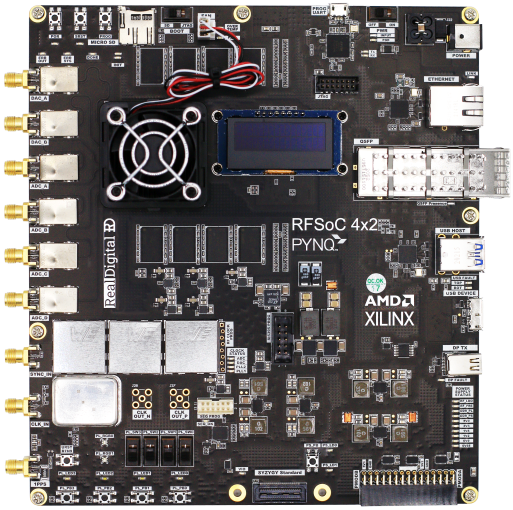
\includegraphics[width=0.6\textwidth]{Setup-software/figures/rfsoc4x2.png}
    \caption{Picture of a RFSoC4x2 board.}
    \label{fig:rfsoc4x2}
\end{figure}

The \RFSoC is much smaller than the \ZCU, while it is smaller, the \RFSoC is a FPGA of third generation, meaning it has much higher sampling frequencies.
Since there are just two DACs, this board can be used to control a single non-flux-tunable qubit. The connections will be:
\begin{itemize}
    \item \textbf{DAC 1:} drive line
    \item \textbf{DAC 2:} readout line
    \item \textbf{ADC 1:} feedback line (for readout)
    \item \textbf{ADC 2:} not active
    \item \textbf{ADC 3:} not active
    \item \textbf{ADC 4:} not active
\end{itemize}
As visible in \cref{fig:rfsoc4x2} \RFSoC has direct connections to SMA cables so it does not require any specific additional connector.
By \textit{not active} I mean that the firmware used never activates it; a different firmware potentially could.

On the other hand, the \ZCU board is a bit more complex. As is visible in \cref{fig:zcu111} there are no SMA connectors and an additional board is needed to convert from the black band connectors (the two band on the left in the figure) to SMAs.
\begin{figure}[ht]
    \centering
    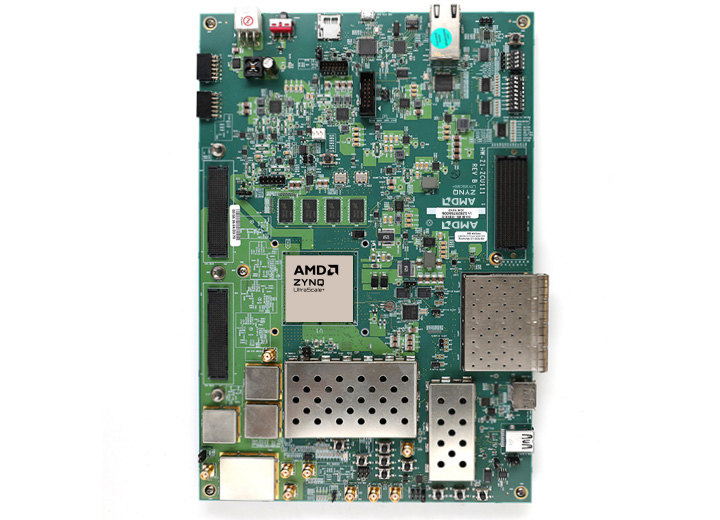
\includegraphics[width=\textwidth]{Setup-software/figures/zcu111.jpg}
    \caption{Picture of a ZCU111 board.}
    \label{fig:zcu111}
\end{figure}

Fortunately, with the \ZCU is sold by default a \textbf{XM500} board, shown in \cref{fig:xm500}.\\
Unfortunately, the \textbf{XM500} board is not just a convertor, but also adds some filtering and changes the output in non trivial ways.
\begin{figure}[ht]
    \centering
    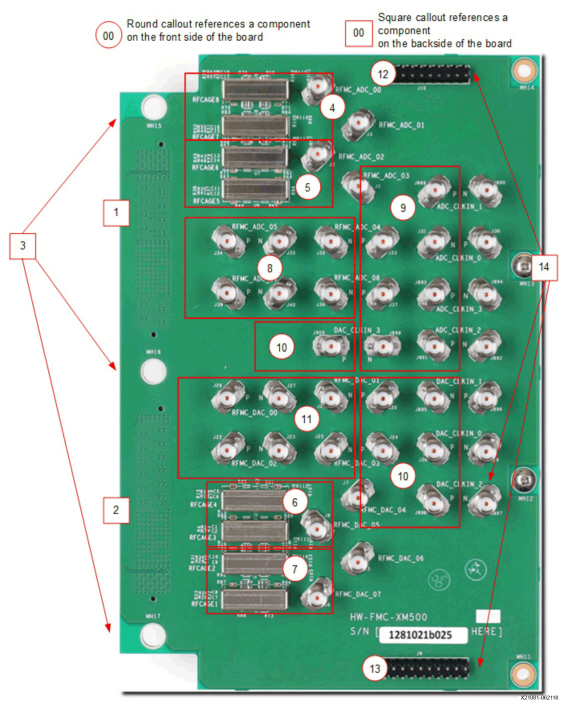
\includegraphics[width=0.65\textwidth]{Setup-software/figures/xm500.jpeg}
    \caption{Picture of a XM500 board.}
    \label{fig:xm500}
\end{figure}
In particular, the \textbf{XM500} has:
\begin{itemize}
    \item \textbf{external clock inputs/outputs:} not active;
    \item \textbf{4 single output DACs:} these are all active, but they have a balun filter added to it. That is a high-pass filter that removes DC components. So these cannot be used for DC flux control;
    \item \textbf{2 ADC:} active and also with baluns (but there are no downsides here);
    \item \textbf{3 differential output DACs:} these do not have baluns, so they can be used for flux lines, but require specific differential amplifiers to subtract the two outputs to convert them to a single SMA (also, the vast majority of differential amplifiers does not work for DC signals).
\end{itemize}

For the \ZCU, the \Qick project offers two different firmwares: one uses both ADCs, so can be used to control up to two flux-tunable qubits, the other uses a single ADC multiplexed.
The multiplex firmware is of particular interest and has been extensively used during the thesis.
Loading it, one of the DACs become capable of sending 4 different pulses at different frequencies but at the same time, while one of the ADC becomes capable of acquiring 4 different pulses (again at 4 different frequencies) at the same time.

This is one of the perks of using a re-configurable FPGA: since the ADCs and DACs are products of the FPGA logic is possible to reconfigure them so that a single ADC is actually composed of 4 with smaller bandwidth.\\
For this configuration, anyway, we used a standard upconversion system for the DAC so that, even with a smaller $f_s$, the output was in the first Nyquist zone (for power reasons).


\subsection{Qubits Configuration}

At TII, the XLD cryostat was used at its full capacity and contained, at the mixing chamber level:
\begin{itemize}
    \item 3 single non-flux-tunable qubit manufactured by TII, in custom 3D cavities;
    \item a 5 flux-tunable qubits chip, with a star connectivity (namely a single qubit in the middle that can couple to the other four);
    \item a 5 flux-tunable qubits with couplers (namely flux-tunable qubits between other qubits, used to mediate the interaction between the two qubits);
    \item  a 25 qubit chip with 5 readout lines and various qubits connected to each other.
\end{itemize}

In the work for this thesis, I tested and interacted, in particular, with the single qubit devices and one readout line of the 25 qubit chip.

The single qubits, that were changed and replaced over my period at TII, generally share the same schematic and the reader can imagine them as presented in \cref{fig:single_qubit}.

\begin{figure}[ht]
    \centering
    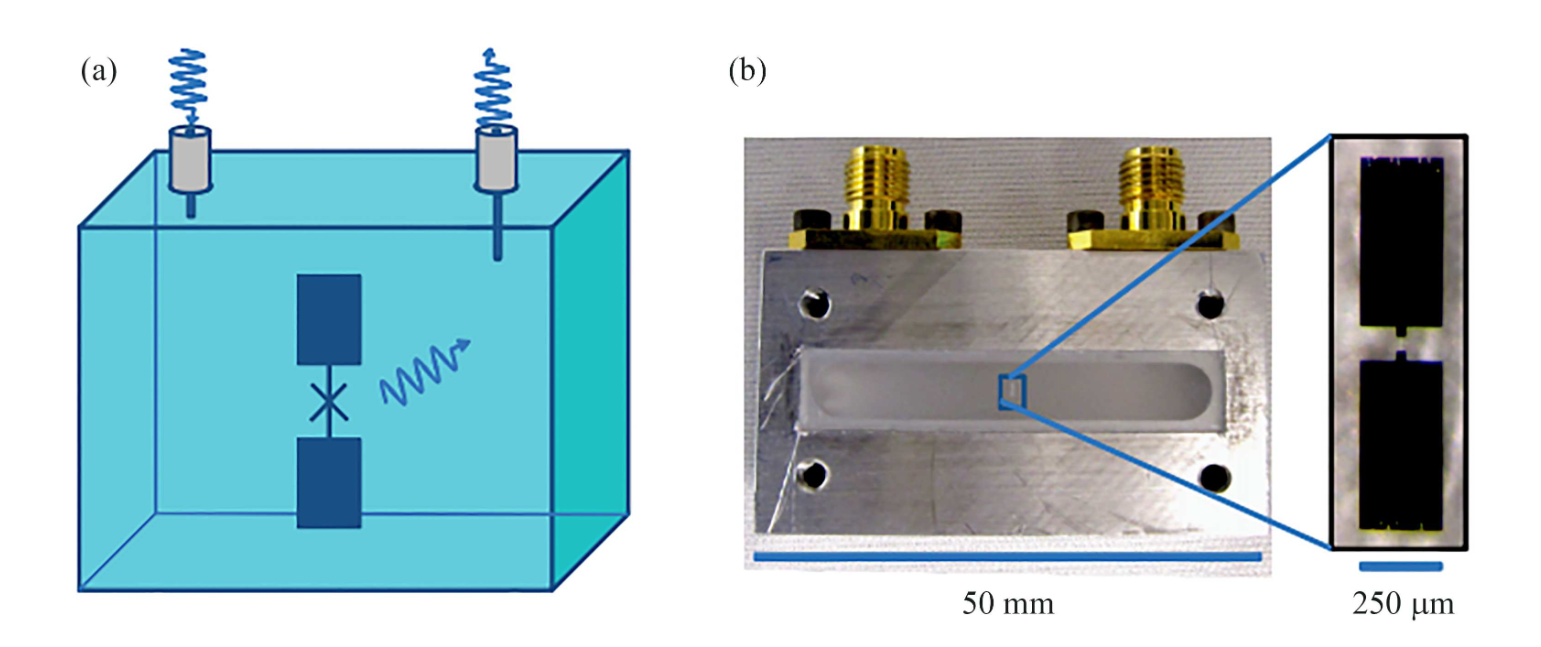
\includegraphics[width=\textwidth]{Setup-software/figures/ex:transmon.png}
    \caption[Example of a single qubit in a 3D cavity]{Example of a single qubit in a 3D cavity. Credits~\cite{Huang2020}.}
    \label{fig:single_qubit}
\end{figure}

\begin{figure}[ht]
    \centering
    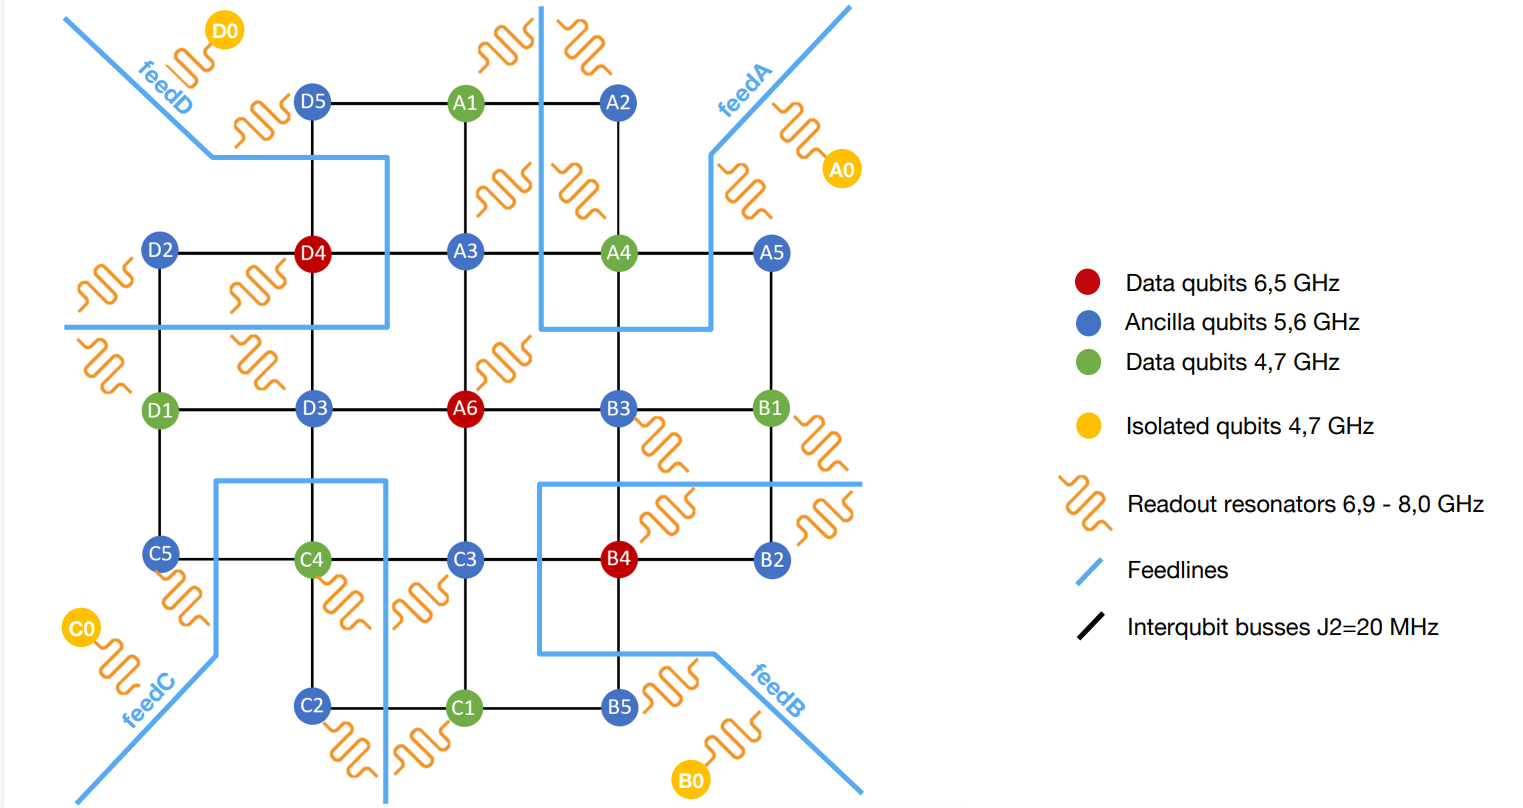
\includegraphics[width=0.8\textwidth]{Setup-software/figures/contralto.png}
    \caption[Topology of the Contralto QuatWare chip]{Topology of the Contralto QuatWare chip. Credits~\cite{contralto}.}
    \label{fig:contraltro_chip}
\end{figure}
The 25 qubits chip is schematically presented in \cref{fig:contraltro_chip}

Among all the present qubits, the \ZCU was connected to line D.\\
Note that every line has 5 qubits plus an isolated one (the yellows) that are qubit used only for testing.\\
Moreover, all the black interconnecting lines are possible two-qubits gates.


\subsection{Configuration and setup for RFSoC4x2}

During this thesis work, the \RFSoC was connected to multiple single qubit in 3D cavities.
Therefore, the setup changed several times, but it always had some stable attributes.
For example, in a single qubit (transmon) non flux tunable, there is only a single line for input (were both readout and drive pulses are fired) and a single readout output (\textit{feedback}).

\begin{figure}[ht]
    \centering
    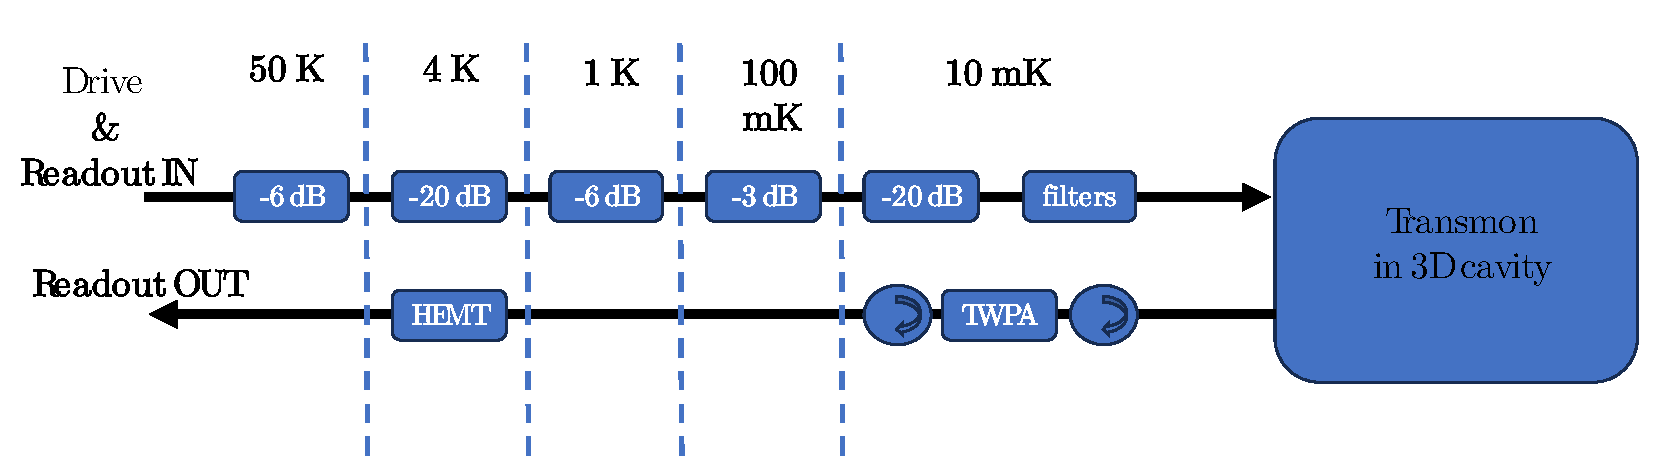
\includegraphics[width=\textwidth]{Setup-software/figures/scheme_lines_single.pdf}
    \caption{Schematics of the lines of a single non-flux-tunable qubit in a 3D cavity.}
    \label{fig:lines_single}
\end{figure}

In \cref{fig:lines_single} the two lines (in-fridge) are presented.
All the attenuation present in the IN line is needed to help to reach the single-photon level (or near-single-photon) and its spread to avoid excessive thermal load to a specific stage of the dilution.\\
The filters represented at the mixing chamber level included both IR filter and low-pass filters to clean in the best possible way any noise.

In the readout OUT line, the first element is TWPA~\cite{Yaakobi2013} manufactured by Silent Waves~\cite{silentwaves} continuously pumped (with another line not present in the scheme) during the experiments.
The role of the TWPA is to amplify the signal, inducing a noise amplification quantum limited.
Note that the TWPA was not present in the majority of the setups, but is inserted in the scheme for completeness.\\
At the $4$ K level, a cryogenic HEMT~\cite{Baulieu2022} is present so that the signal, extremely low in the input, becomes measurable.

At room temperature the \textit{feedback signal} is amplified with a LNA (Low Noise Amplifier) manufactured by MiniCircuit~\cite{minicircuit} (max $+8$ dB ) and sent to the \RFSoC ADC 0.\\
The drive source is DAC 0 (B on the board) and sometimes an amplification of max $+8$ dB was needed.
The readout IN was connected to DAC 1 (A on the board) and merged to the drive by using a passive \textit{splitter}.\\
At room temperature, some band-pass filters were added to remove spurious created by the synthesis process and eventual high frequency noise.


\subsection{Configuration and setup for ZCU111}

Similarly as per single qubit control, in \cref{fig:lines_zcu} are showed the in-fridge lines for the control of the multiplexed qubits of the 25 qubits chip. 

\begin{figure}[ht]
    \centering
    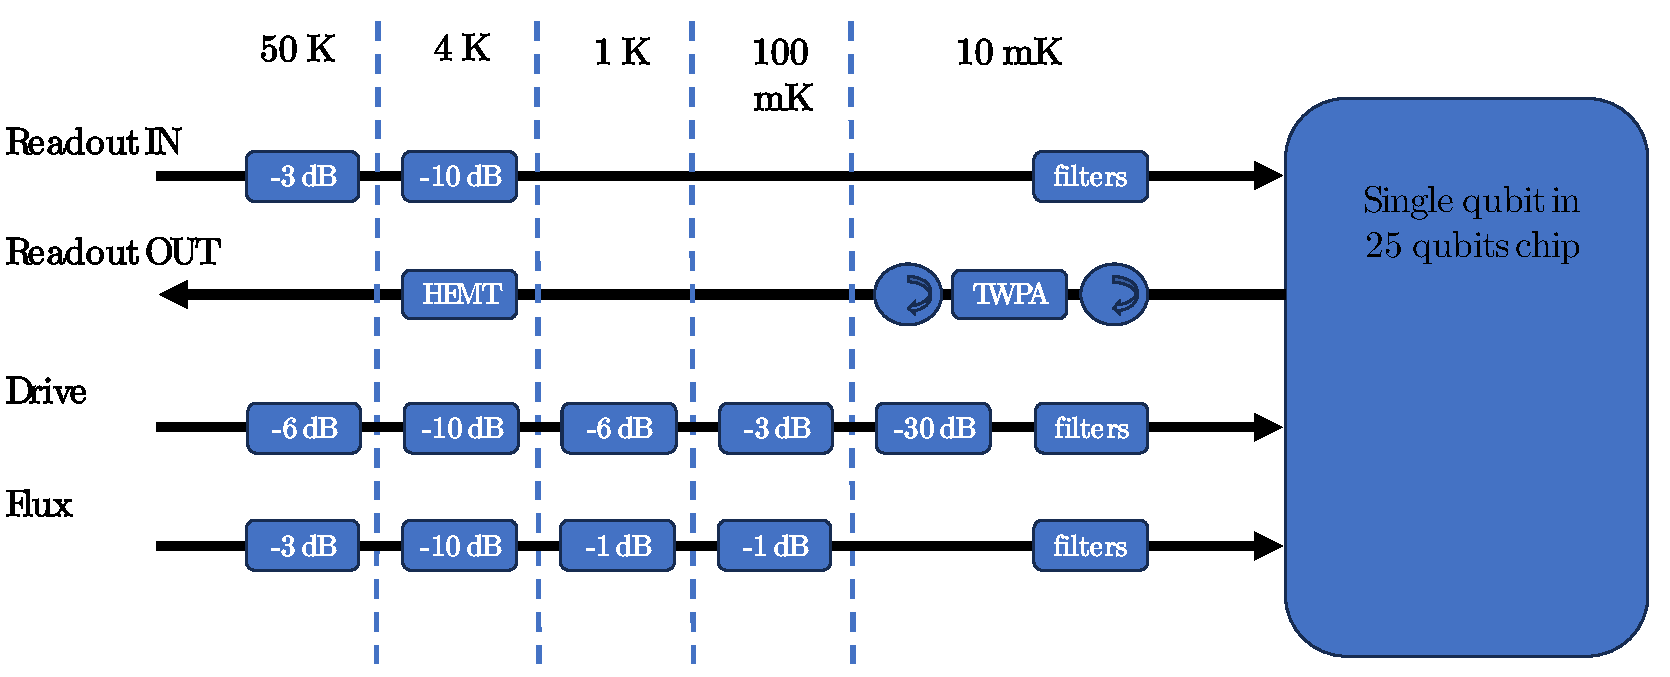
\includegraphics[width=\textwidth]{Setup-software/figures/scheme_lines_25.pdf}
    \caption{Schematics of the lines of a single flux-tunable qubit in the 25 qubit chip.}
    \label{fig:lines_zcu}
\end{figure}

Note first that there are multiple input lines and, in particular, that the readout in and the drive line are are separated.
This is mainly because this is a 2D chip and not a cavity.\\
In any case, both for the readoutIN and the drive the filters are the same already named in the single qubit setup.

For the flux line, on the other hand, the filters are extremely low frequency filters since in theory we just need a DC current.

The TWPA is one of the differing elements. In fact it was not used a standard fixed-band TWPA as per the single qubit setup, but a prototype of a variable-band TWPA~\cite{Ranadive2022}.
This TWPA needs a pump to work and a DC current to tune the amplification band and gain. Both these lines are not showed in the scheme since they are more or less secondary.

Some more differences are present at room temperature, where the setup is a bit more complex.
In particular note that the schematics presented in \cref{fig:lines_zcu} represent a single qubit, but this is a system with 5+1 multiplexed qubits.
Therefore, at room temperature we will have the DAC 6 of the \ZCU connected to the readoutIN while a mux firmware is loaded.
This basically cause the bandwidth to go from $6$ GHz to few MHz, is therefore required a local oscillator with an up-conversion scheme as presented in \cref{fig:up-down-conversion}. 
\begin{figure}[ht]
    \centering
    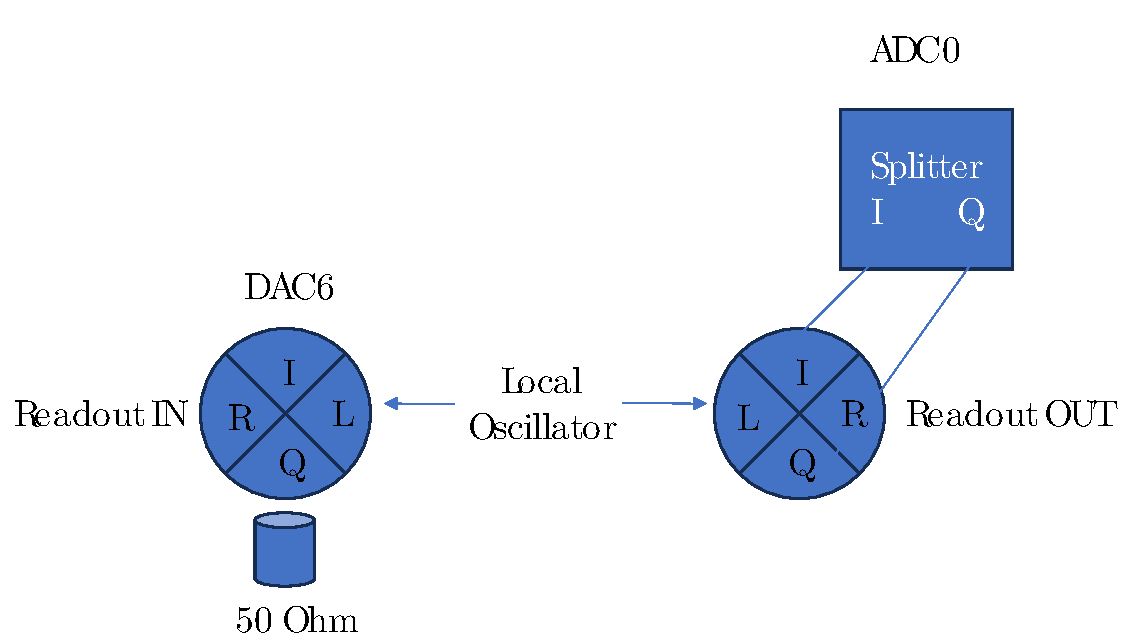
\includegraphics[width=0.7\textwidth]{Setup-software/figures/upconversion.pdf}
    \caption{Scheme used for down and up-conversion.}
    \label{fig:up-down-conversion}
\end{figure}
As it shown, the same local oscillator is also used for down-conversion.
Since this process uses an IQ mixer, in the down-conversion I and Q are splitted and gets merged back again using a splitter connected to the board ADC 0.

For the drive lines is sometimes needed additional amplification that was provided through a LNA.
They were connected to DAC 3-4-5 to achieve full control of 3 qubits at the same time.

For the flux lines some more work is needed since the outputs of the companion XM500 board (that exposes the SMA connections) have baluns (i.e. DC filters) on its single-ended connection.
There are two option to proceed: it is possible to buy/project a new companion boards or to leverage the 3 differential outputs of the XM500.
This second option was chosen for simplicity.
Note that the differential outputs P-N can be merged together via a simple subtraction P-N, something that standard differential amplifiers easily do, but that since we are aiming for DC currents these are not an option because they use capacitors and operates as high-pass filters.
Special active differential amplifiers are needed in this case.\\
Having bought 3 of them, we were able to bias 3 flux-tunable qubits using DACs 0-1-2.

\subsection{Configuration and setup for ZCU216}

The \textbf{ZCU216} was used with the same setup composed for the \textbf{ZCU111}.
This was a temporary solution that was also limiting the board potential.

In particular, the \textbf{ZCU216} could potentially be used to fully control 7 flux tunable qubits (considering 7 drive lines, 7 flux lines and a maximum of 2 readout inputs), while with the used scheme only three qubits were usable.
To fully unblock the board potential, however, it is needed to make some changes to the \Qick firmware and this requires particular work.

